\section{Nested TBMD optimization and Pareto regimes}
\label{sec:optimization}
Train-only rank selection reduces the original full-state pressure and saturation RMSE from \OptRepOriginalPressure/\allowbreak\OptRepOriginalSaturation{} to \OptRepJointPressure/\allowbreak\OptRepJointSaturation{} for joint ranks $(80,48,2,32)$. Independent property factors yield a lower equal-property normalized objective, but POD-E remains better for pressure alone. The accuracy and compression TBMD representations store \OptAccuracyCompression{} and \OptCompressionCompression{} times fewer values than rank-32 POD-E. Detailed rank, conditioning and ablation curves are in Supplementary Section~S7.

At all 30 existing joint wells, POD-E retains the lowest pressure and saturation errors (Table~\ref{tab:optimization_main}). Optimizing recovery on the original basis cannot remove its representation floor. Independent property models become poorly conditioned under sparse joint-well sensing, so their full-observation advantage does not imply a sparse advantage. Pressure-only measurements favour TBMD for pressure (\OptPressureWellThirtyCompressionPressure{} versus \OptPressureWellThirtyPodePressure{} $u_p$), while the independent saturation coefficients remain unobserved.

\begin{table}[htbp]\centering\small
\caption{Nested P2 reconstruction from all 30 existing joint-property wells (60 scalar channels); the prior uses no observations. Values are mean $\pm$ sample standard deviation over ten scenarios. Pressure uses export unit $u_p$ and saturation is dimensionless. Compression is the POD-E/TBMD factor-storage ratio. Bold marks the automatically determined smallest mean; method labels denote train-selected configurations.}
\label{tab:optimization_main}
\setlength{\tabcolsep}{3pt}
\begin{adjustbox}{max width=\textwidth}
\begin{tabular}{lrrr}\toprule
Method & Pressure RMSE & $S_o$ RMSE & Compression \\ \midrule
POD-E random & \textbf{0.084 $\pm$ 0.027} & \textbf{0.00057 $\pm$ 0.00013} & 1.00$\times$ \\
POD-E & \textbf{0.084 $\pm$ 0.027} & \textbf{0.00057 $\pm$ 0.00013} & 1.00$\times$ \\
Joint TBMD (tuned ranks) & 0.089 $\pm$ 0.023 & 0.00064 $\pm$ 0.00013 & 1.22$\times$ \\
TBMD compression & 0.175 $\pm$ 0.083 & 0.00065 $\pm$ 0.00012 & 2.62$\times$ \\
TBMD optimized & 0.179 $\pm$ 0.046 & 0.00064 $\pm$ 0.00013 & 2.12$\times$ \\
POD & 0.216 $\pm$ 0.123 & 0.00076 $\pm$ 0.00026 & 1.00$\times$ \\
Prior + IDW & 0.313 $\pm$ 0.165 & 0.00078 $\pm$ 0.00020 & -- \\
Original TBMD + tuning & 0.429 $\pm$ 0.051 & 0.00423 $\pm$ 0.00003 & 3.11$\times$ \\
Prior & 1.148 $\pm$ 0.558 & 0.00084 $\pm$ 0.00021 & -- \\
\bottomrule\end{tabular}\end{adjustbox}\end{table}


At 100 grid channels, optimized independent TBMD lowers the normalized joint error to \OptGridHundredAccuracyJoint{} from POD-E's \OptGridHundredPodeJoint. At 300 channels, the compressed model reaches \OptGridThreeHundredCompressionJoint{} versus \OptGridThreeHundredPodeJoint, with a lower joint objective in all ten folds. Pressure error remains higher; the gain is driven by saturation. Thus POD-E is preferred for existing joint wells and pressure accuracy, while TBMD offers a conditional accuracy--storage trade-off (Fig.~\ref{fig:opt_pareto}). Corrected cluster-constrained placement and all candidate baselines remain in the supplementary registry; clustering does not improve the 30-channel comparison.

\begin{figure}[tbp]
\centering
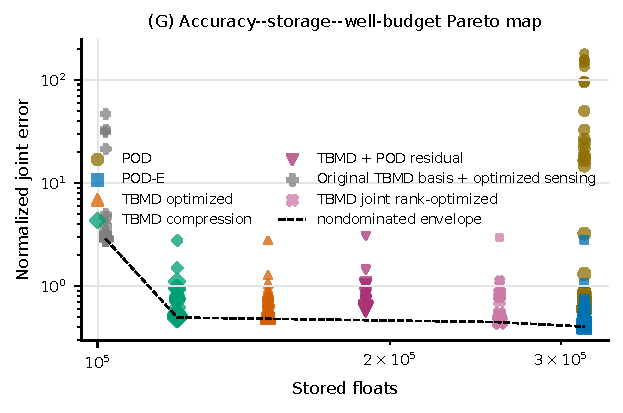
\includegraphics[width=\textwidth]{../../../studies/brugge_sparse_sensing/figures/fig14_pareto.pdf}
\caption{Accuracy--storage--well-budget map. Marker size increases with well budget; the dashed envelope contains nondominated mean points within the joint-well regime.}
\label{fig:opt_pareto}
\end{figure}
